\chapter{Processo e tecniche di sviluppo per applicazioni MR per Hololens2}
\pagestyle{plain}
In questa sezione andremo a vedere come inizializzare un progetto Unity e utilizzare l'MRTK al suo interno. Successivamete si andrà ad approfondire entrambi, andando a vedere il funzionamento dei componenti utilizzati in questo progetto e le tecniche di programmazione utilizzate. 


\section{Setup di Unity}
\subsection{Installazione di Unity}
Andare nel sito ufficiale di Unity e scaricare l'ultima versione disponibile. Dopo l'installazione ci si troverà davanti all'Unity Hub, qui la schermata potrebbe leggermente cambiare a seconda della versione ma delle opzioni 3d disponibili \textbf{non} bisogna scegliere la versione \textbf{URP} o \textbf{HDRP} ma la versione normale \textbf{3D}. 
\begin{figure}[H]
    \centering
    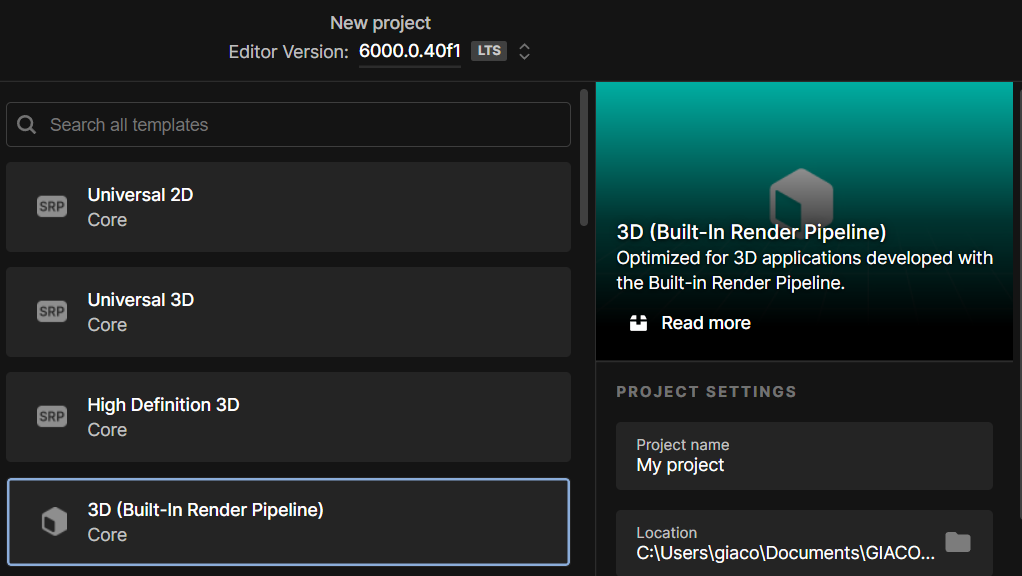
\includegraphics[width=0.9\textwidth,height=\textheight,keepaspectratio]{figures/chapter_1/unityHub.png}
    \caption{In questo caso la versione corretta è quella selezionata}
\end{figure}
Dopo aver dato nome al progetto e selezionata la cartella di installazione andiamo subito a modificare le impostazioni di build.
\begin{figure}[H]
    \centering
    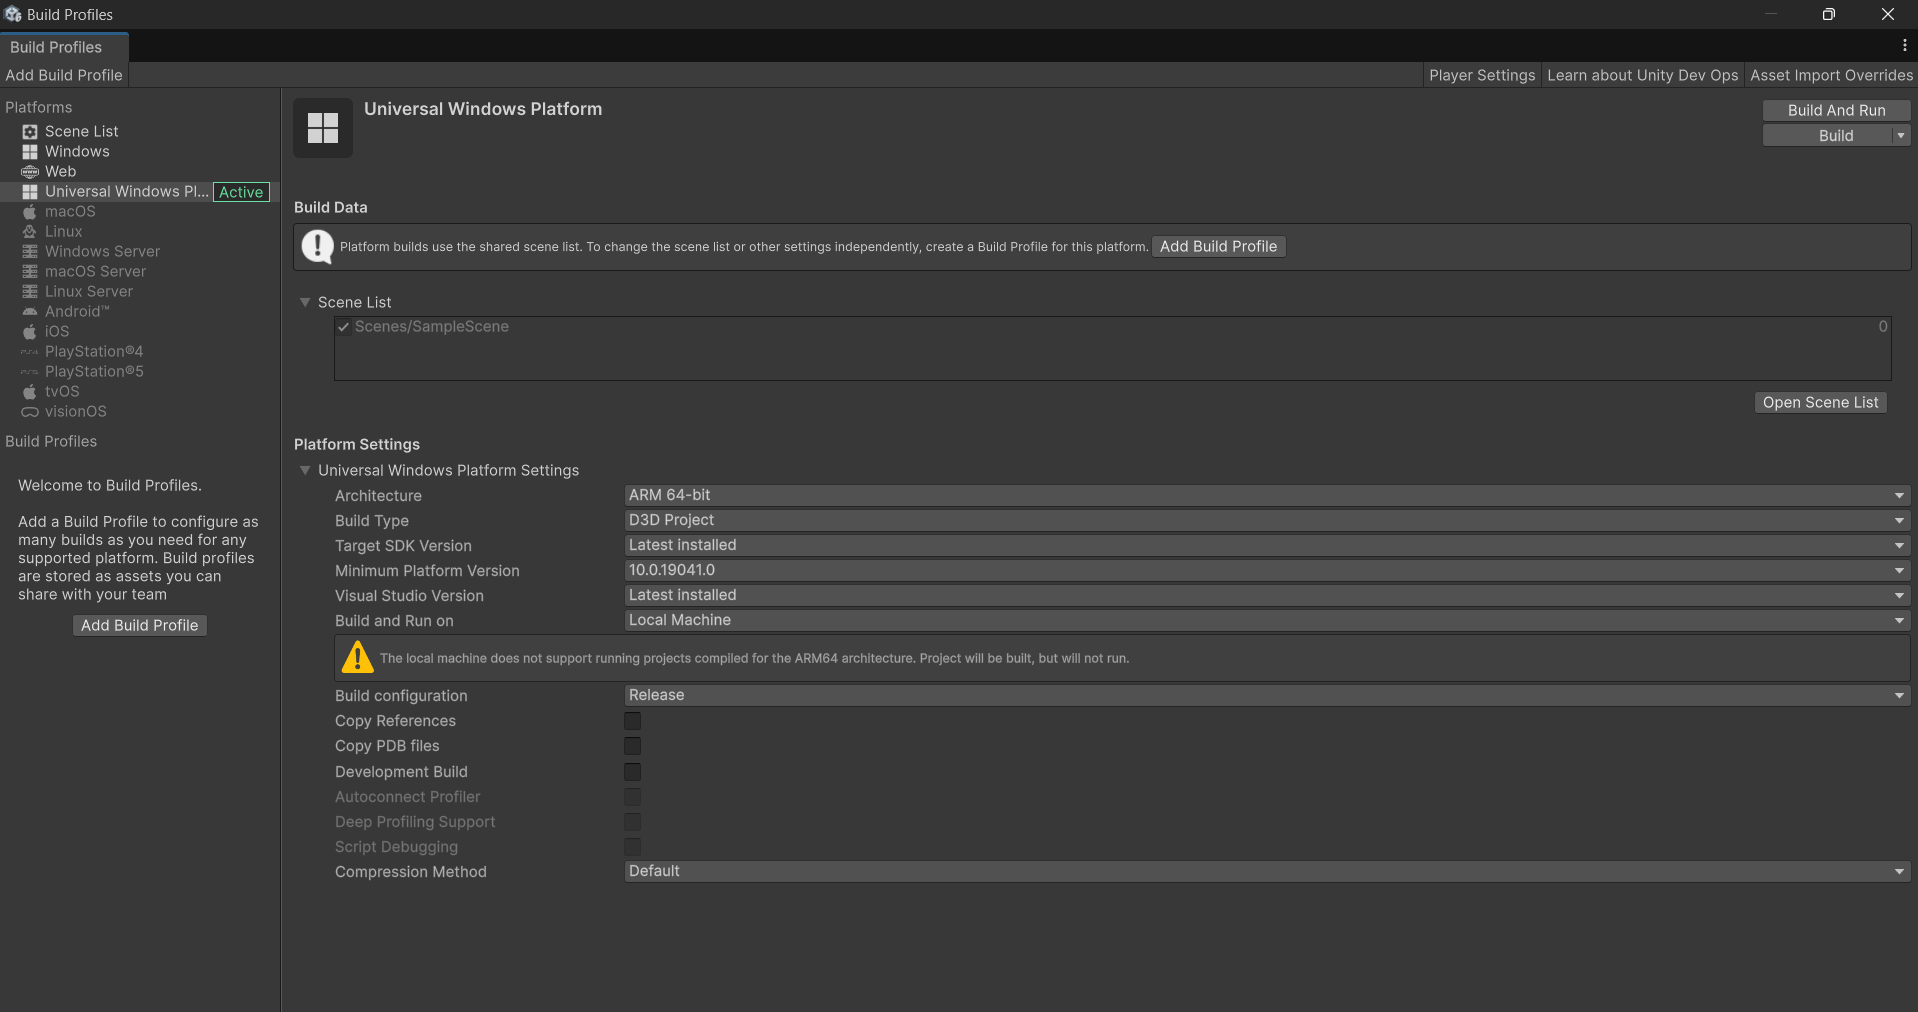
\includegraphics[width=0.9\textwidth,height=\textheight,keepaspectratio]{figures/chapter_1/impostazioniBuild.png}
    \caption{Da notare il "Build Type"}
\end{figure}
Prima di tutto bisogna essere sicuri di aver attivato la build per l'Universal Windows Platform e di aver selezionato la piattaforma \textbf{ARM64} come architettura, questo è fondamentale per il corretto funzionamento dell'applicazione su Hololens2, poi bisogna essere sicuri di avere come build type \textbf{D3D}.
\subsection{Installazione di Mixed Reality Feature Tool}
Dopo questi passaggi scaricare il "Mixed Reality Feature Tool" dal sito ufficiale di Microsoft, questo strumento ci permette di scaricare e installare l'MRTK (Mixed Reality Toolkit) direttamente all'interno del nostro progetto. Una volta scaricato, aprire l'eseguibile, selezionare il path del progetto Unity, nella schermata successiva selezionare tutta la sezione "MRTK3" e alla sezione "Platform Support" selezionare "Mixed Reality OpenXR Plugin". 
\begin{figure}[H]
    \centering
    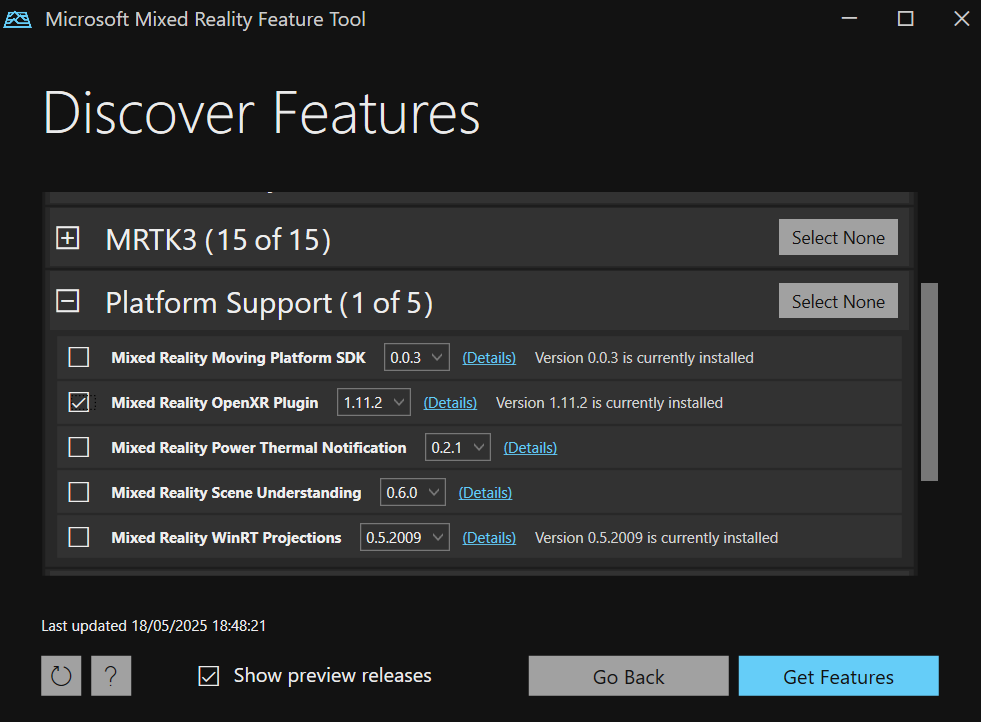
\includegraphics[width=0.9\textwidth,height=\textheight,keepaspectratio]{figures/chapter_1/mixedRealityTool.png}
    \caption{}
\end{figure}
Dopo ciò ritornare su Unity e aspettare che il pacchetto venga importato.
\subsection{Impostazioni del progetto e della scena}
 Una volta completata l'installazione dei pacchetti andare nelle impostazione del progetto e seguire le seguenti immagini:
\begin{figure}[H]
    \centering
    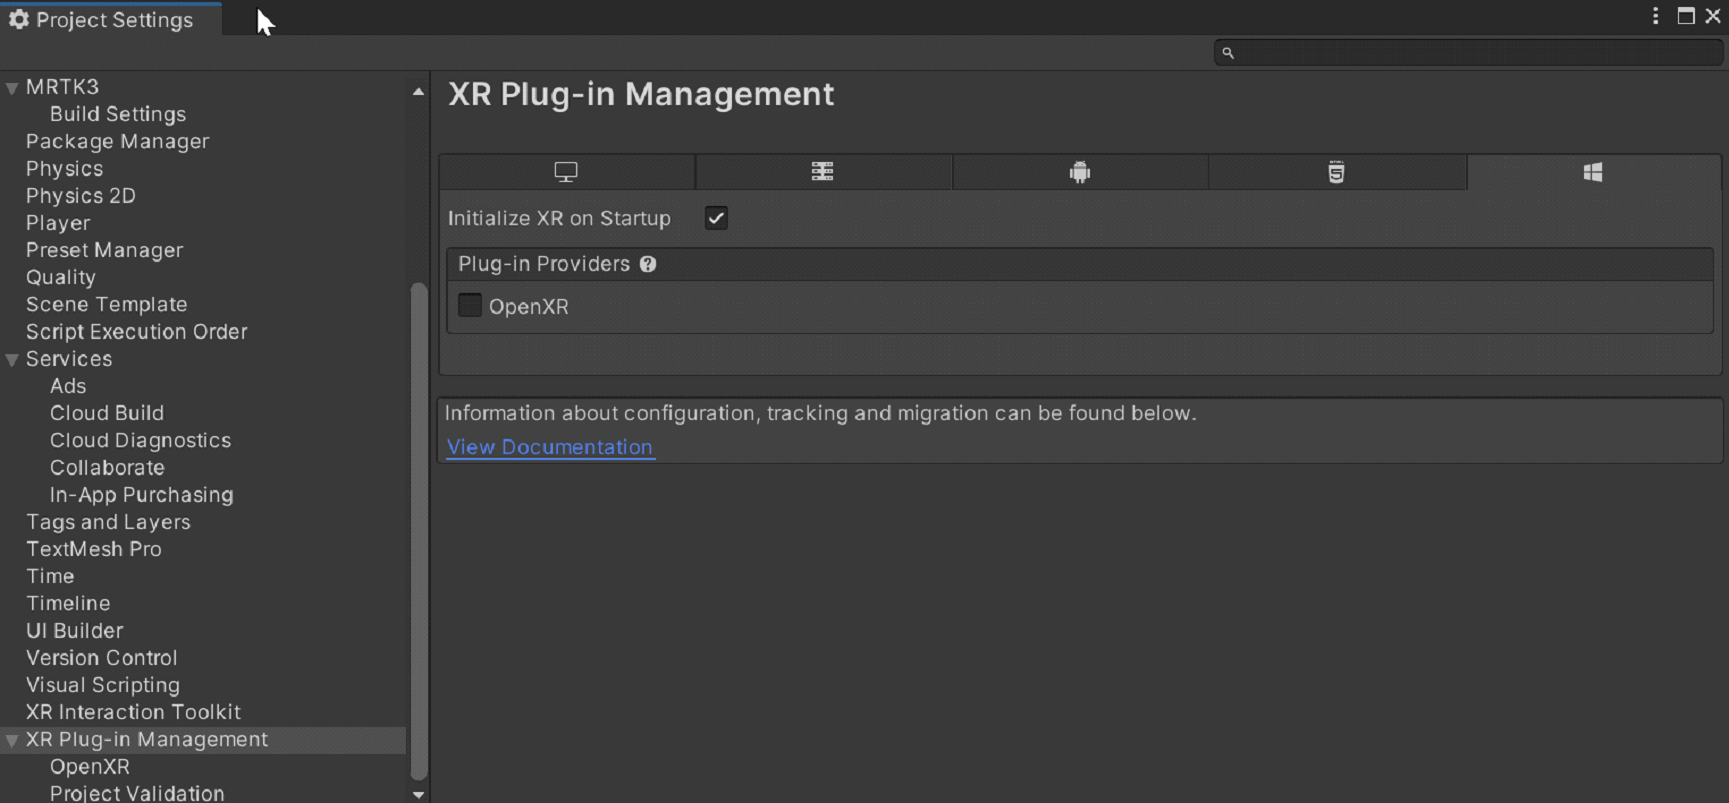
\includegraphics[width=0.9\textwidth,height=\textheight,keepaspectratio]{figures/chapter_1/projectSetting1.png}
    \caption{Andare nelle impostazioni del progetto e selezionare la sezione "XR Plug-in Management"}
\end{figure}
\begin{figure}[H]
    \centering
    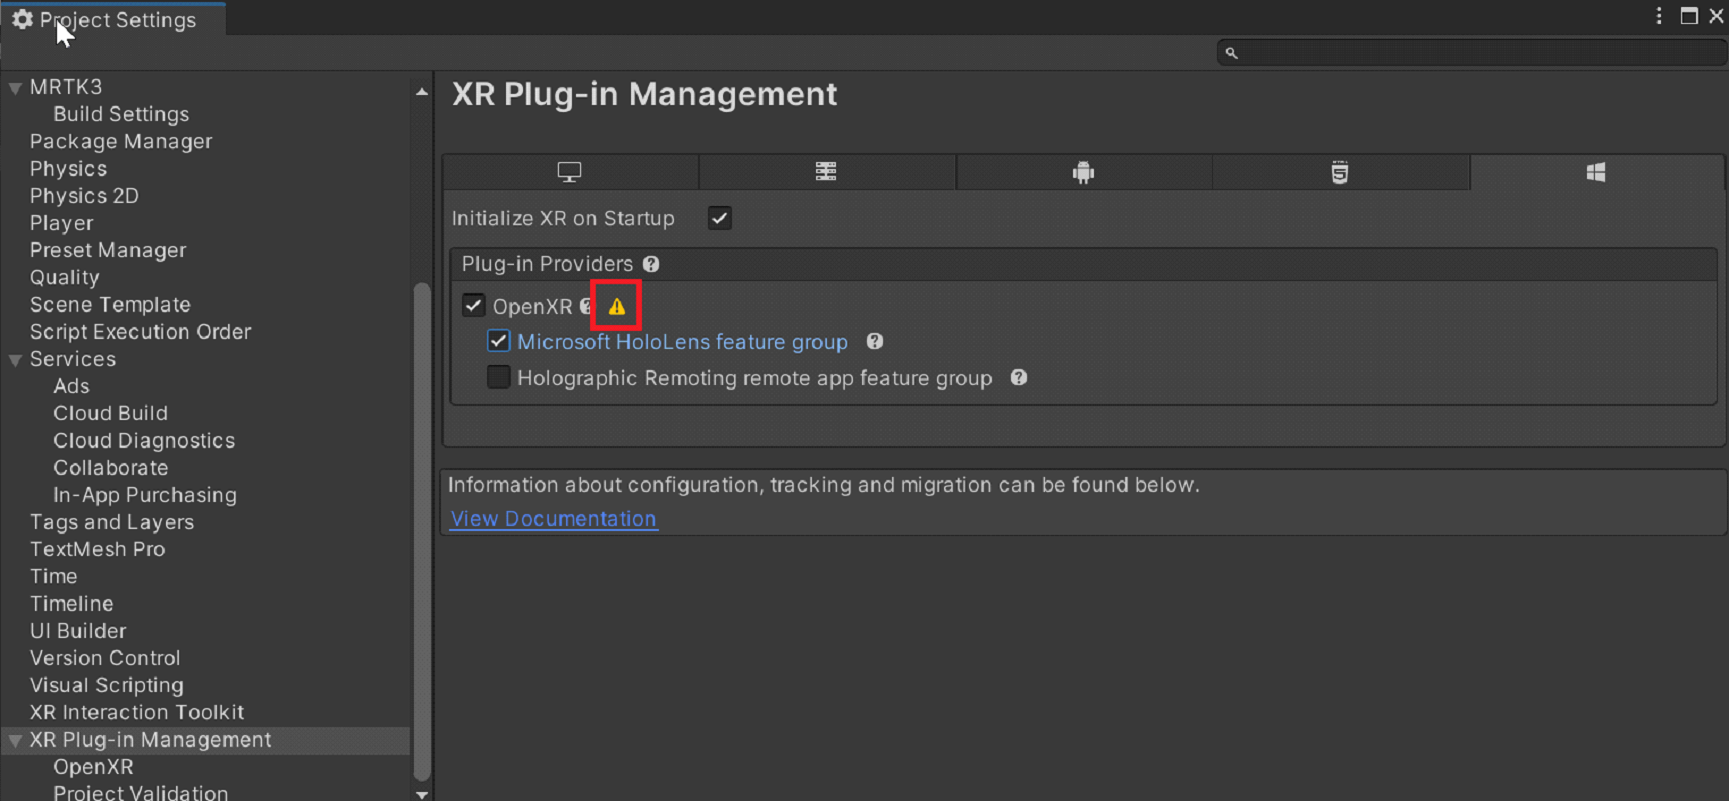
\includegraphics[width=0.9\textwidth,height=\textheight,keepaspectratio]{figures/chapter_1/projectSetting2.png}
    \caption{Abilitare l'OpenXR}
\end{figure}
\begin{figure}[H]
    \centering
    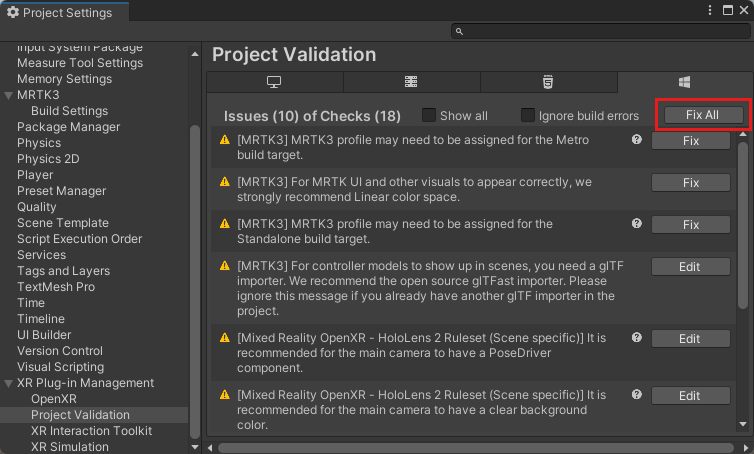
\includegraphics[width=0.9\textwidth,height=\textheight,keepaspectratio]{figures/chapter_1/projectSetting3.png}
    \caption{Se compare il triangolo giallo, cliccarci sopra e premere "Fix All"}
\end{figure}
\begin{figure}[H]
    \centering
    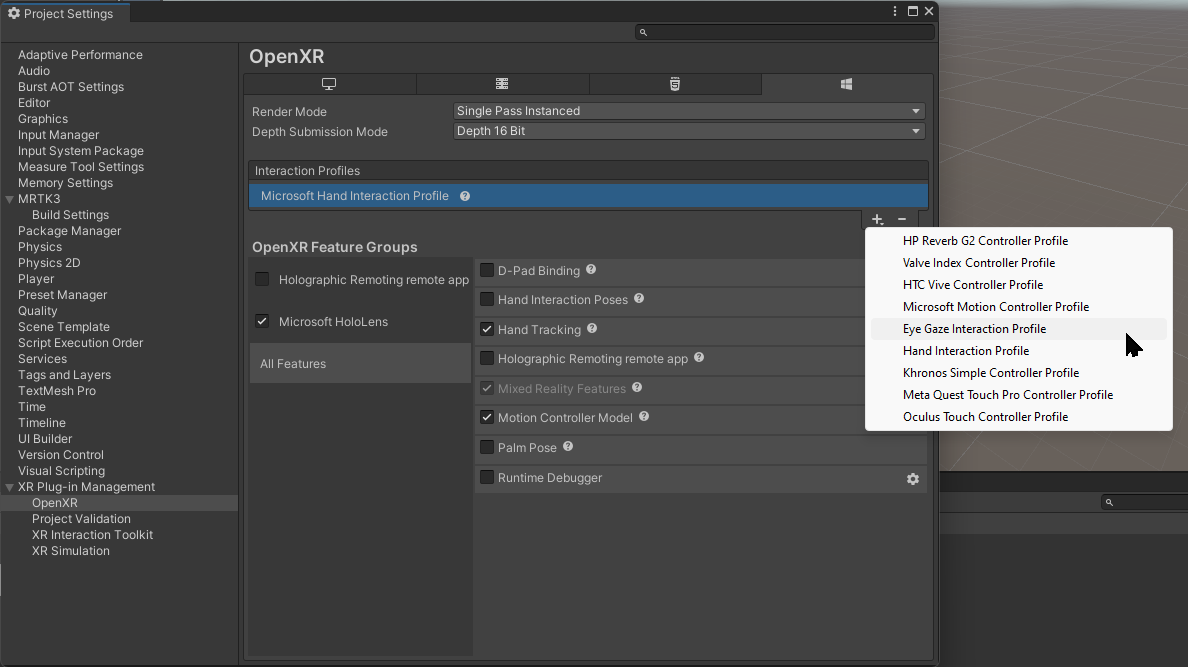
\includegraphics[width=0.9\textwidth,height=\textheight,keepaspectratio]{figures/chapter_1/projectSetting4.png}
    \caption{Inserire i seguenti profili e abilitare le spunte in foto}
\end{figure}
\begin{figure}[H]
    \centering
    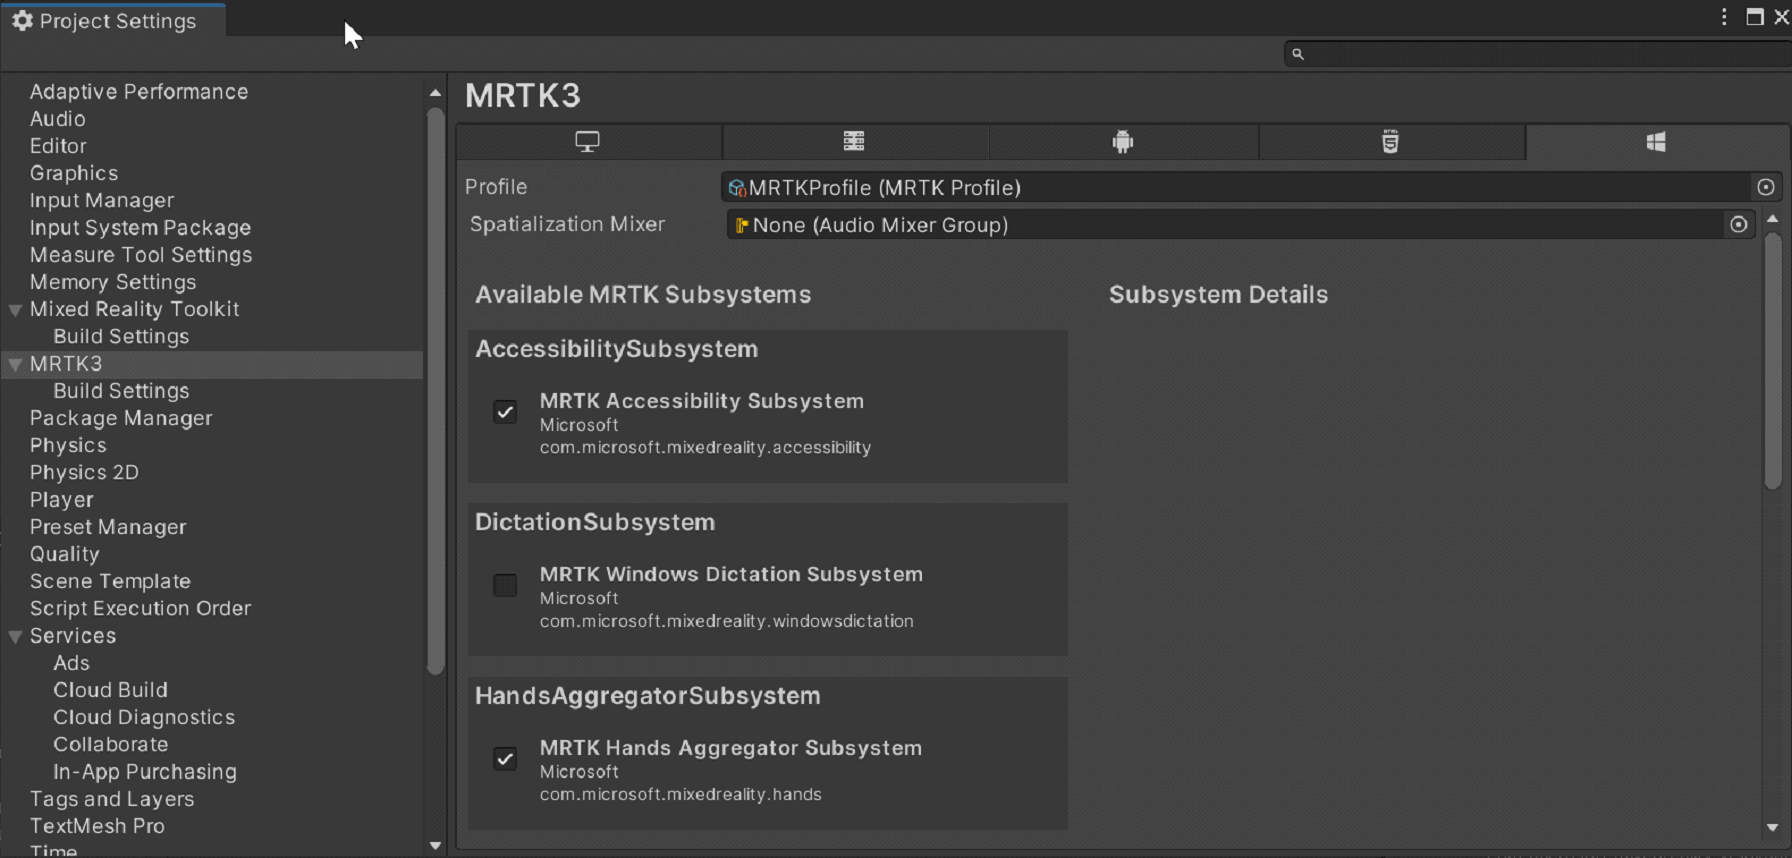
\includegraphics[width=0.9\textwidth,height=\textheight,keepaspectratio]{figures/chapter_1/projectSetting5.png}
    \caption{Nella sezione MRTK3 selezionare il profilo come in figura}
\end{figure}
Una volta completati questi passaggi tornare alla scena principale di Unity, andare nella sezione che mostra le gerarchia degli oggetti ed eliminare tutto, poi andare nella sezione in basso denominata "Project", navigare dentro "Pakages" -> "MRTK Input" -> "Assets" -> "Prefabs", trovare "MRTK XR Rig" e trascinarlo nella scena.
\begin{figure}[H]
    \centering
    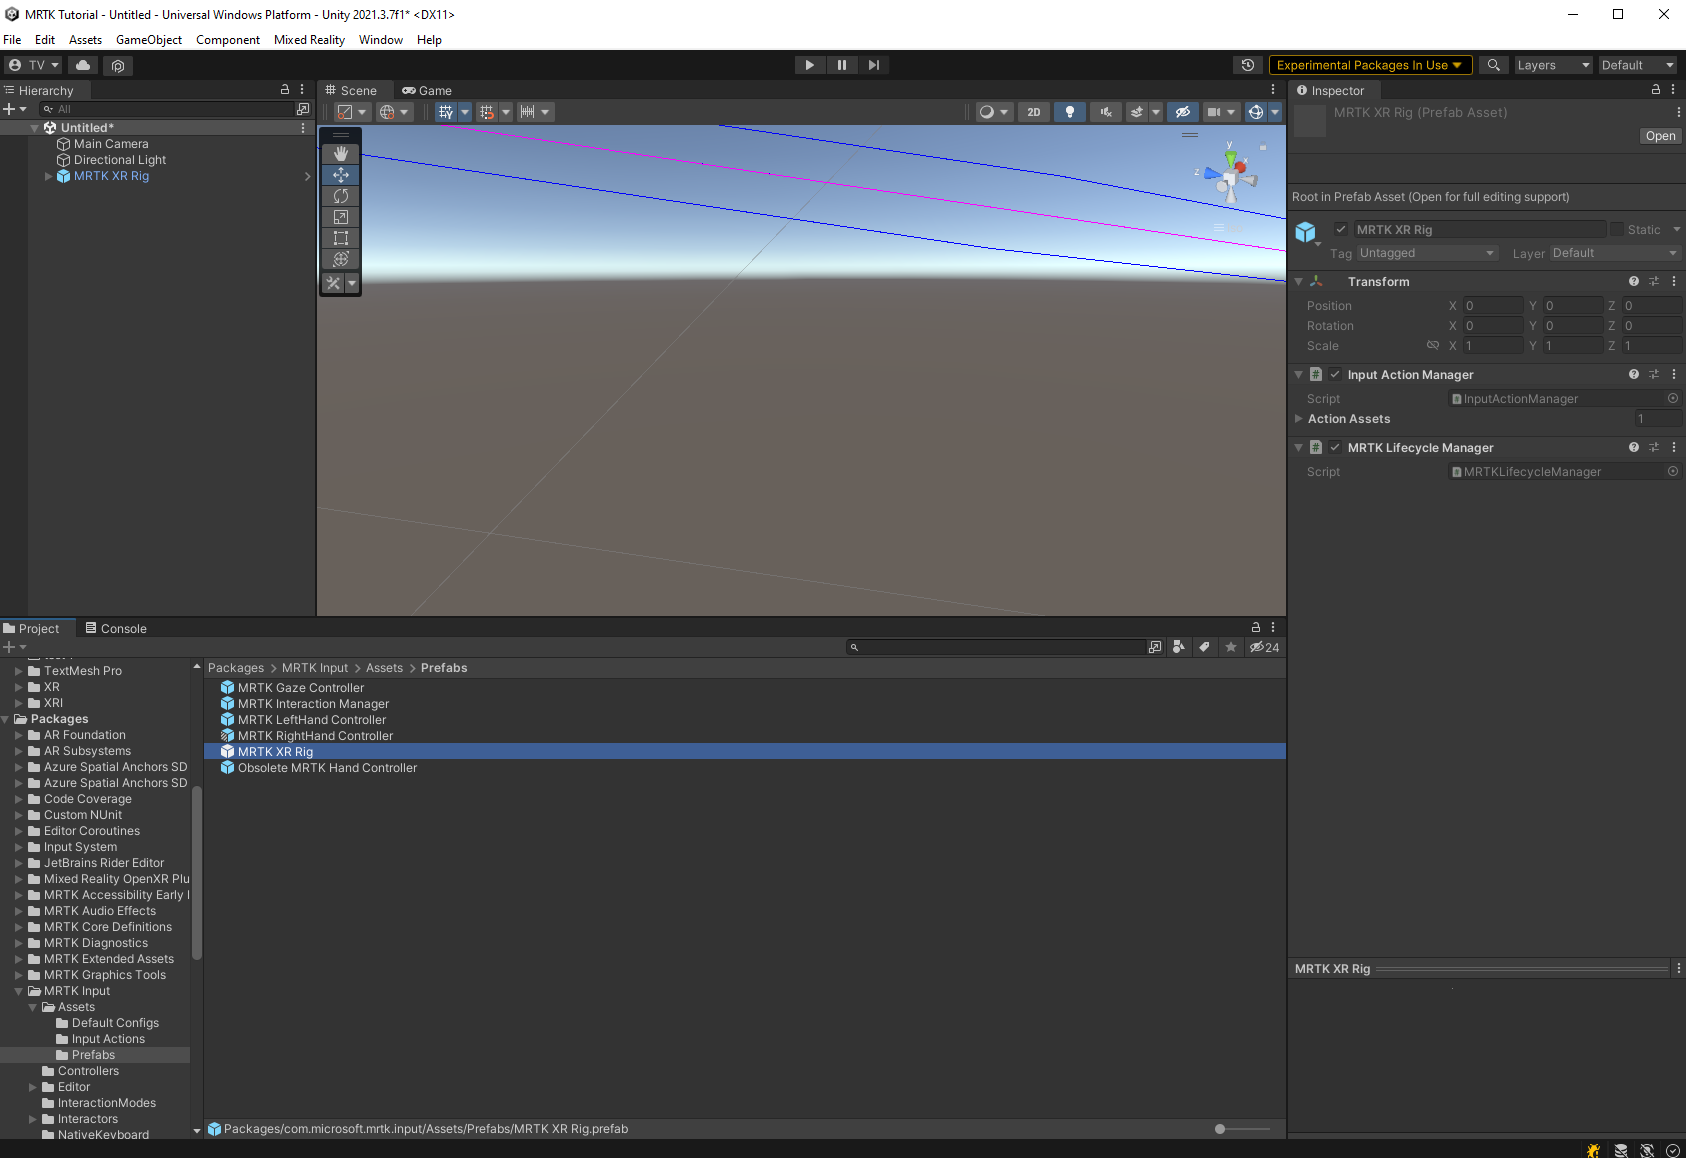
\includegraphics[width=0.9\textwidth,height=\textheight,keepaspectratio]{figures/chapter_1/mrtk-xr-rig-prefab.png}
    \caption{}
\end{figure}
Fare la stessa cosa con "MRTK Input Simulator" che si trova in "Packages" -> "MRTK Input" -> "Simulation" -> "Prefabs".
Con questo il setup di Unity è completo, ora possiamo iniziare a lavorare con l'MRTK e a sviluppare la nostra applicazione.
\section{MRTK3.0}
Andiamo a vedere i principali componenti utilizzati in questo progetto e il loro funzionamento.
\subsection{Tabs}
Questo componente è stato utilizzato per visualizzare le tre ricette generate da Gemini e, nella Slate principale, per separare la foto scattata dalla lista di ingredienti rilevati dall'AI.

\begin{figure}[H]
    \centering
    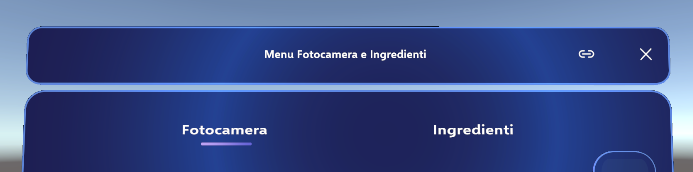
\includegraphics[width=0.5\textwidth,height=\textheight,keepaspectratio]{figures/chapter_1/tabs1.png}
    \caption{Tabs nel menu della fotocamera e ingredienti}
\end{figure}

\begin{figure}[H]
    \centering
    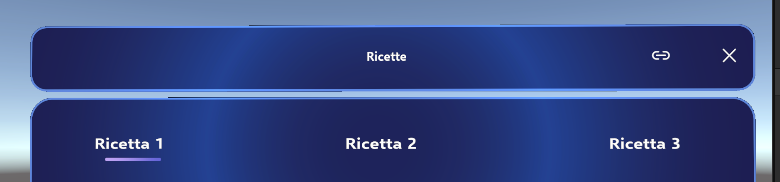
\includegraphics[width=0.5\textwidth,height=\textheight,keepaspectratio]{figures/chapter_1/tabs2.png}
    \caption{Tabs nel menu delle ricette}
\end{figure}
Per creare un menu di Tabs dobbiamo avere due o più bottoni e dei relativi contenuti che verranno nascosti e mostrati a seconda del tab selezionato.
\begin{figure}[H]
    \centering
    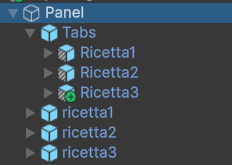
\includegraphics[width=0.4\textwidth,height=\textheight,keepaspectratio]{figures/chapter_1/tabs-gerarchia.png}
    \caption{Gerarchia dei oggetti}
\end{figure}

Gli elementi denominati "Ricetta1", "Ricetta2" e "Ricetta3" sono i bottoni che rappresentano le singole tab, mentre "ricetta1", "ricetta2" e "ricetta3" sono i contenuti che verranno mostrati quando si seleziona il rispettivo tab. Per fare ciò dobbiamo avere il seguente componente nel GameObject Tabs:

\begin{figure}[H]
    \centering
    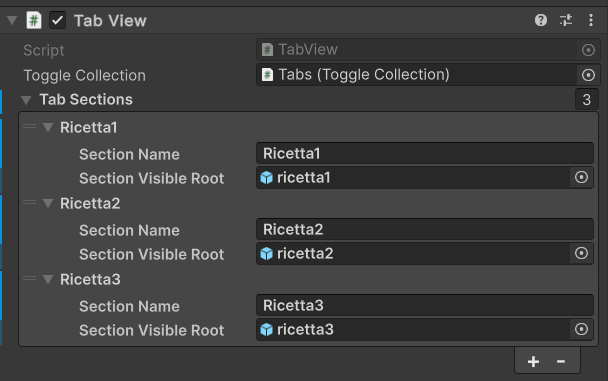
\includegraphics[width=0.4\textwidth,height=\textheight,keepaspectratio]{figures/chapter_1/componente-tabs.png}
    \caption{Componente per il funzionamento delle tabs}
\end{figure}

 In "Toggle Collection" andiamo a trascinare il GameObject padre "Tabs", collezione dei tre bottoni, e in "Tab Selections" andiamo a impostare gli oggetti da visualizzare quando si premono i bottoni. Da notare che l'ordine in cui abbiamo messo i bottoni nel padre "Tabs" è lo stesso ordine in cui andremo a mettere gli oggetti da visualizzare nel componente, quindi il primo bottone mostrerà il primo oggetto e così via. \cite{MRTKtabs}

\subsection{Scroll list}
La scroll list utilizzata in questo progetto è un prefab che si trova all'interno dei pakages dell'MRTK3, precisamente in "MRTK UX Components" -> "Experimental" -> "Scrollable". Se apriamo il prefab la gerarchia di GameObject è la seguente:

\begin{figure}[H]
    \centering
    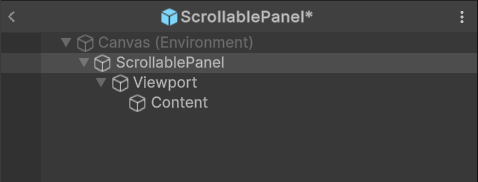
\includegraphics[width=0.4\textwidth,height=\textheight,keepaspectratio]{figures/chapter_1/GerarchiascrollPanel.png}
    \caption{Gerarchia del prefab ScrollablePanel}
    \label{fig:scrollablePanel}
\end{figure}

In Content andiamo a mettere gli oggetti che vogliamo visualizzare e scorrere, Viewport, con i suoi componenti, ci permette di visualizzare solo una parte del contenuto se questo è più grande della finestra di visualizzazione, mentre nell'oggetto ScrollablePanel c'è il componente che ci permette di scorrere il contenuto e definisce la scroll list. 
\begin{itemize}
    \item \textbf{Content}: è consigliabile che abbia un componente come un Grid Layout Group o un Vertical Layout Group, in modo da avere una disposizione ordinata degli oggetti al suo interno.
    \item \textbf{Viewport}: è l'oggetto che contiene il contenuto visibile della scroll list, quindi è fondamentale che abbia un componente Rect Mask 2D, in modo da mascherare il contenuto che esce dalla finestra di visualizzazione.
    \item \textbf{Scrollable Panel}: è l'oggetto che contiene il componente Scroll Rect, a cui dobbiamo assegnare il viewport e le due barre di scorrimento se presenti. In questo modo possiamo scorrere il contenuto all'interno della finestra di visualizzazione. Oltre ad altri componenti c'è anche "Scrollable", dove dobbiamo impostare la "Scroll Rect" ed è un componente dell'MRTK3
\end{itemize}

\begin{figure}[H]
    \centering
    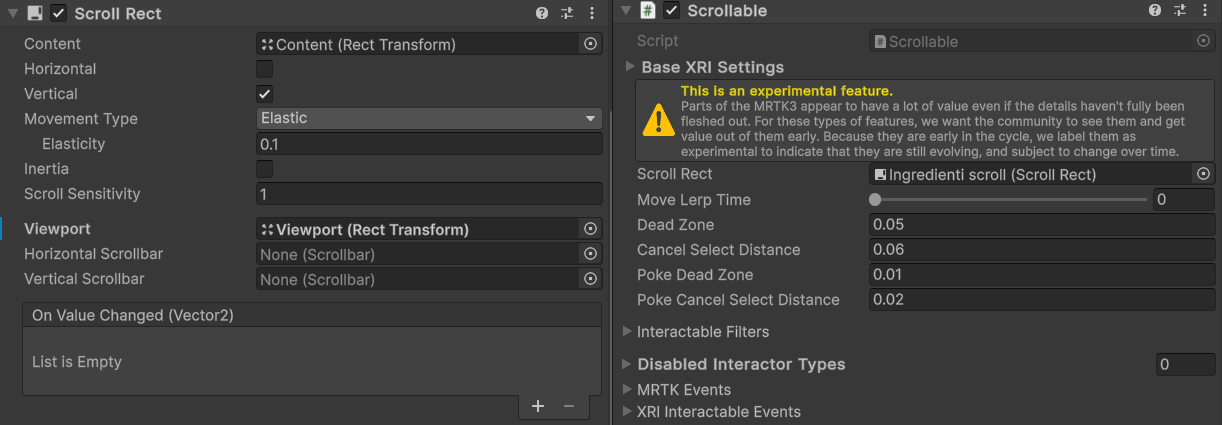
\includegraphics[width=0.8\textwidth,height=\textheight,keepaspectratio]{figures/chapter_1/ComponentiScrollBar.png}
    \caption{Componenti per \textbf{Scrollable Panel}}
\end{figure}

\subsection{Slate}
La Slate offre una finestra che consente la visualizzazione di contenuti 2D, come testo, immagini e elementi grafici come bottoni e menu, come una vera e propria finestra di una applicazione desktop. La Slate è un oggetto prefab che si trova all'interno dei pakages dell'MRTK3, precisamente in "MRTK UX Components (Non-Canvas)" -> "Slates".

\begin{figure}[H]
    \centering
    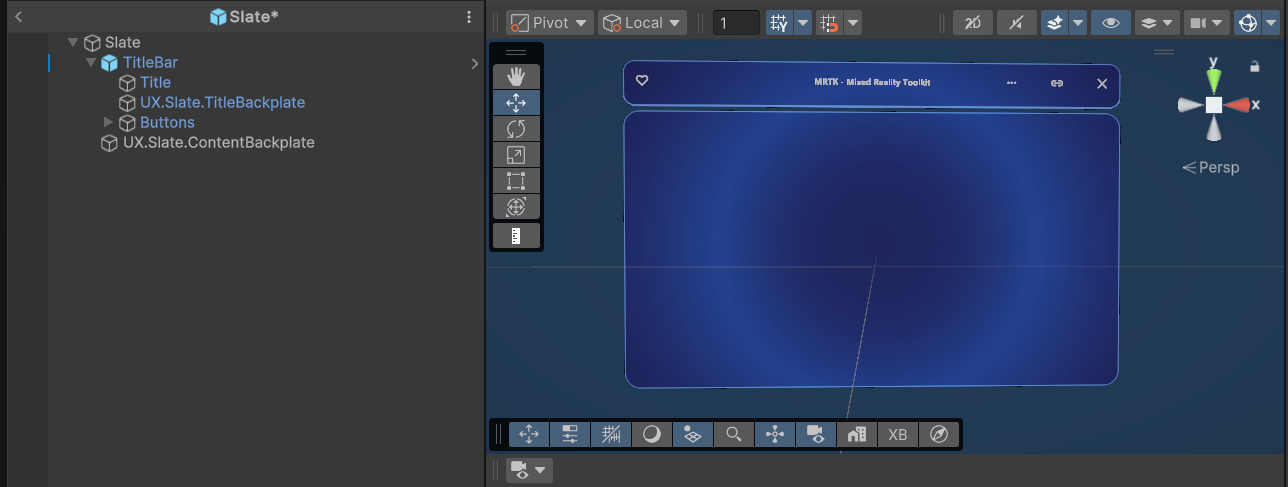
\includegraphics[width=0.8\textwidth,height=\textheight,keepaspectratio]{figures/chapter_1/slate.png}
    \caption{Gerarchia e UI della Slate}
\end{figure}

La Slate è composta principalmente da:
\begin{itemize}
    \item \textbf{TitleBar}: è la barra in alto, ha due bottoni personalizzabili, altri due bottoni per chiudere la finestra e abilitare il follow e il titolo.
    \item \textbf{UX.Slate.ContentBackplate}: il contenitore padre dove andremo a mettere gli oggetti che vogliamo visualizzare all'interno della finestra
\end{itemize}

La Slate può essere trascinata dove si vuole prendendola dalla TitleBar, può essere chiusa e si può abilitare il follow, in modo che segua la posizione dell'utente.
\cite{MRTKslate}

\subsection{Near Menu}
Il Near Menu offre un menù che può essere spostato o può seguire l'utente, in modo tale da non dare fastidio alle interazioni con gli altri elementi. Il Near Menu lo possiamo trovare sotto forma di Prefab all'interno dei pakages dell'MRTK3, precisamente in "MRTK UX Components" -> "Near Menu".

\begin{figure}[H]
    \centering
    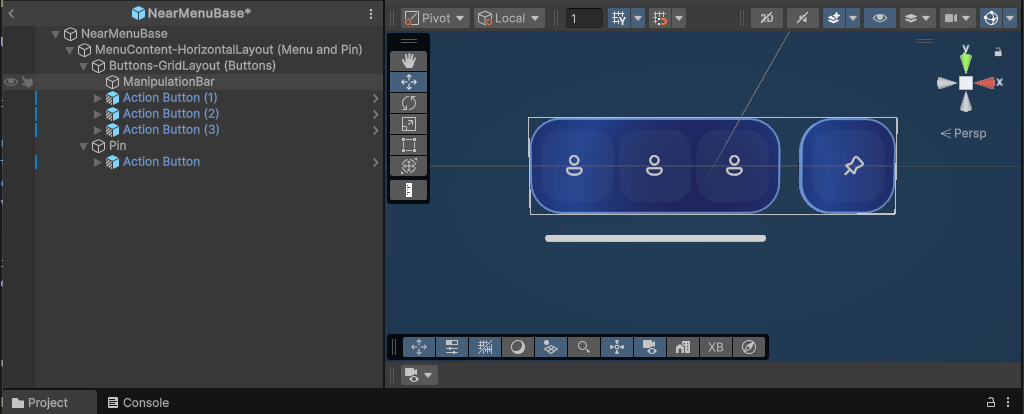
\includegraphics[width=0.8\textwidth,height=\textheight,keepaspectratio]{figures/chapter_1/nearMenu.png}
    \caption{Gerarchia e UI del Near Menu}
\end{figure}

Il Near Menu è composto principalmente da:
\begin{itemize}
    \item \textbf{Bottoni}: Si trovano all'interno di un Grid Layout e ne possiamo aggiungere quanti vogliamo, anche creando più righe e colonne.
    \item \textbf{PinButton}: è il bottone che permette di fissare il menù nella posizione in cui si trova, disattivando il follow
    \item \textbf{ManipulatorBar}: è la barra bianca in basso che permette di prendere e spostare il menù
\end{itemize}

Comportamenti principali del Near Menu:
\begin{itemize}
    \item \textbf{Tag-along}: il menù segue l'utente ponendosi ad una distanza di 30-60cm 
    \item \textbf{Pin}: usando il bottone del pin, situato nella parte più a destra, si fissa il menù nella posizione in cui si trova e si disattiva il follow
    \item \textbf{Grab and move}: essendo il menù un oggetto prendibile e spostabile, si può riposizionare in qualsiasi punto dello spazio prendendolo dalla barra bianca in basso
\end{itemize}

\cite{MRTKnearMenu}

\section{Programmazione in Unity con C\#}
\subsection{MonoBehaviour}
\begin{wrapfigure}{r}{0.50\textwidth} %this figure will be at the right
    \centering
    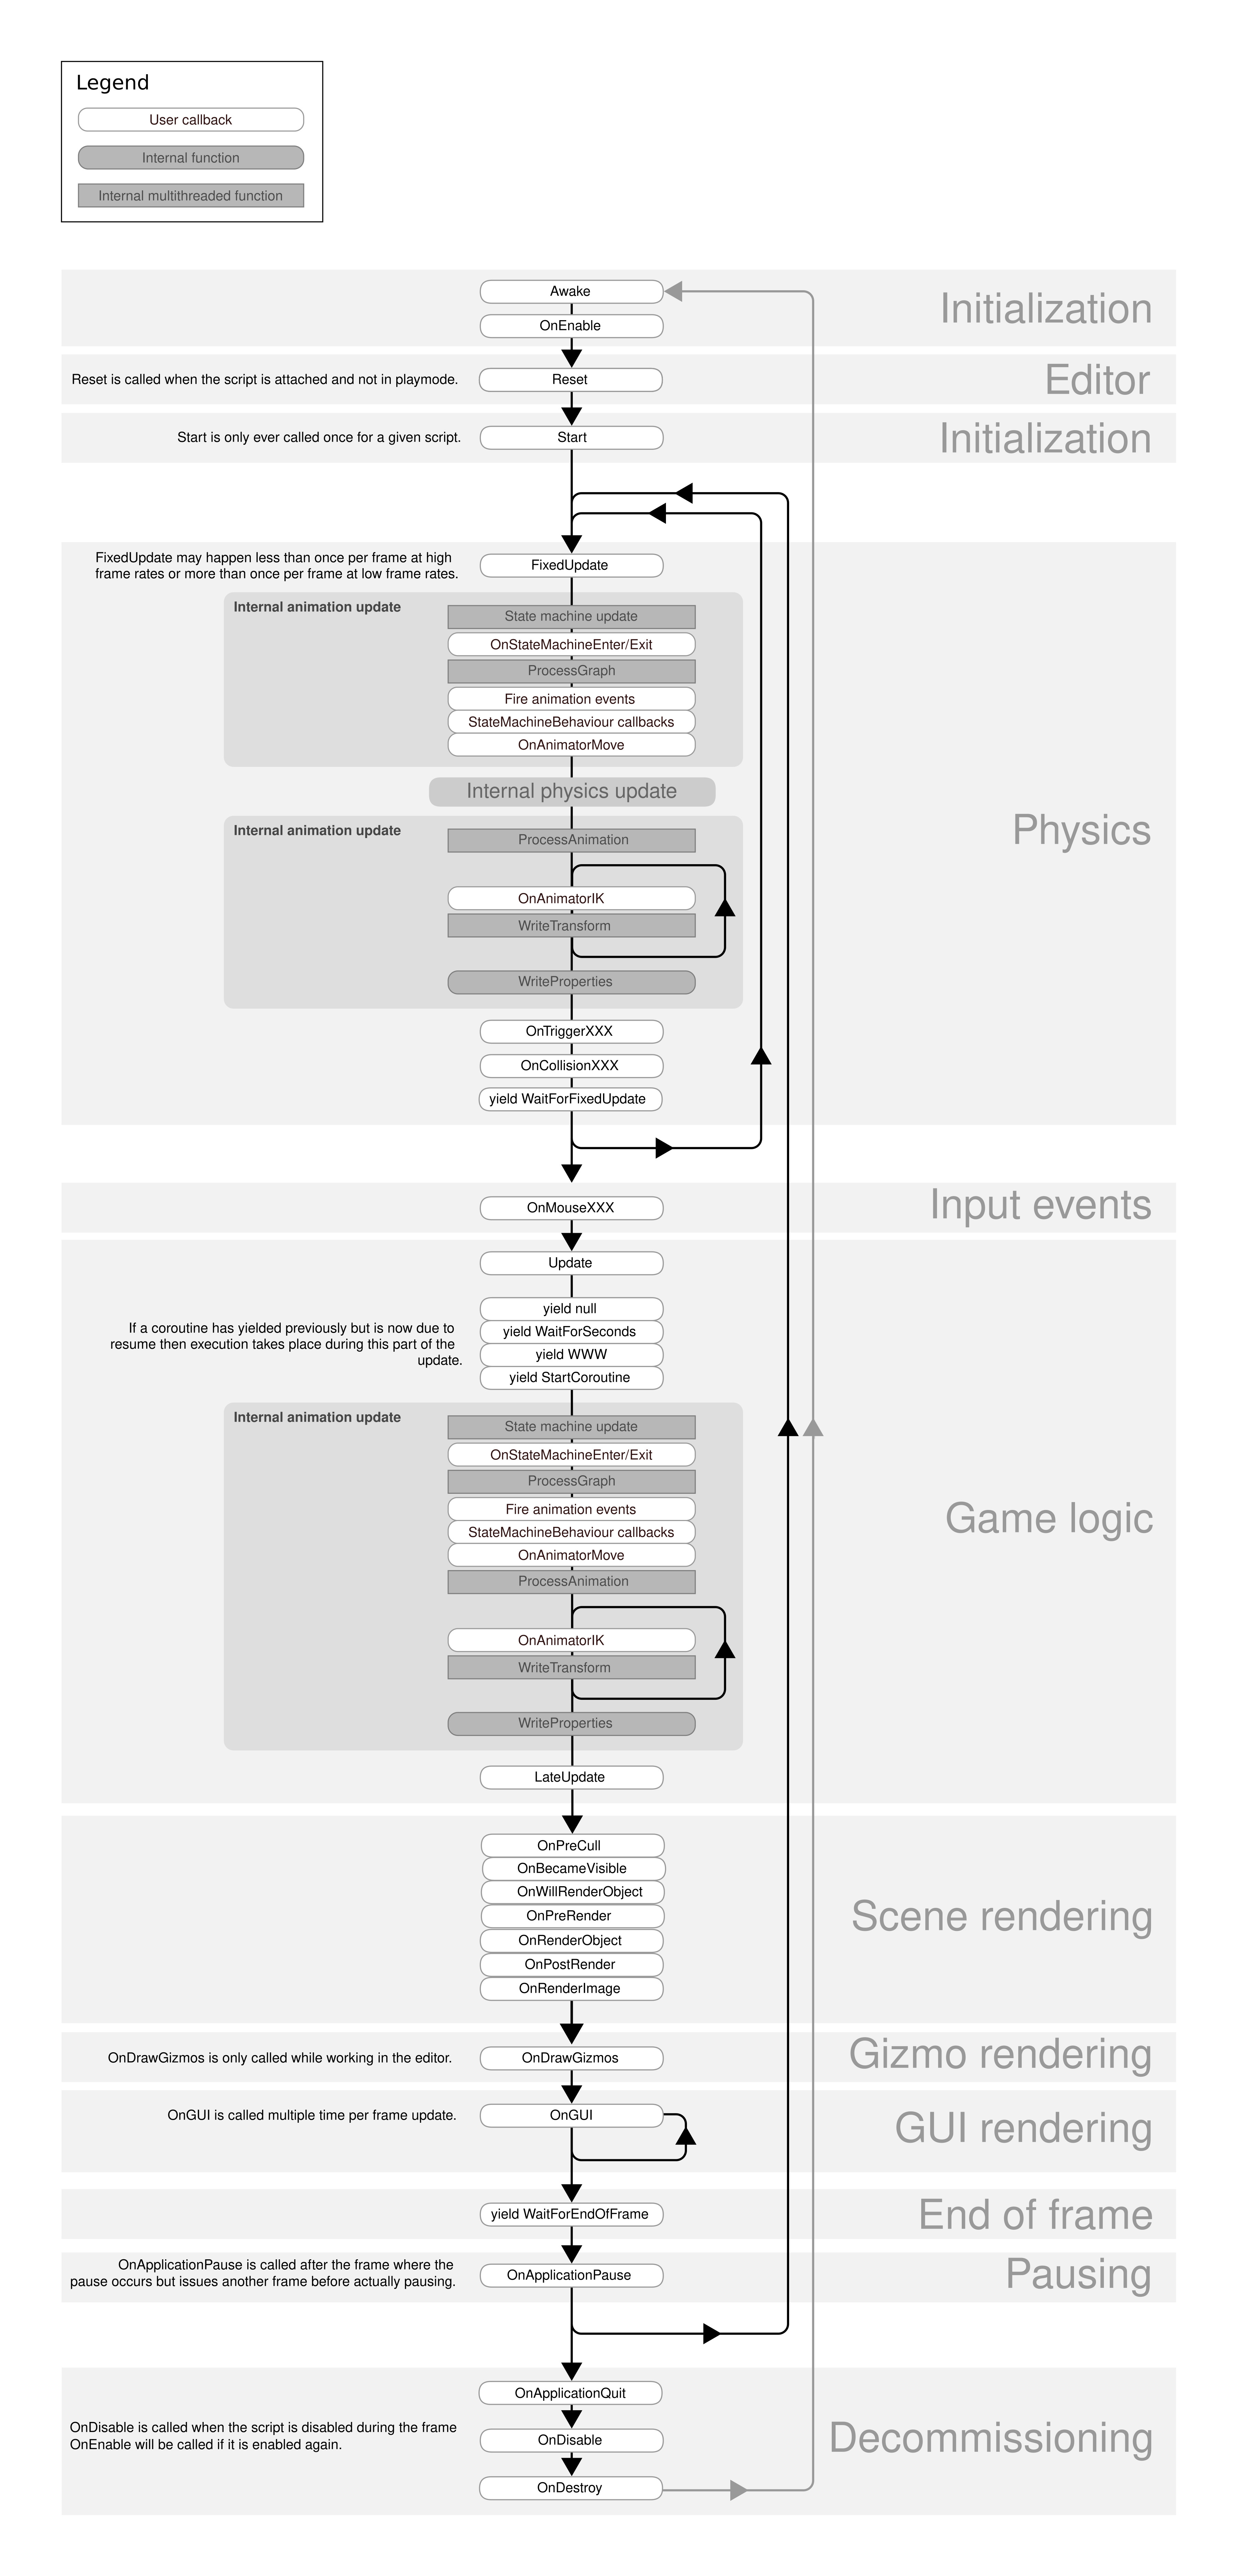
\includegraphics[width=0.40\textwidth]{figures/chapter_1/monobehaviour_flowchart.jpg}
\end{wrapfigure}
Il MonoBehaviour è la classe base da cui derivano tutti gli script in Unity. Quando creiamo uno script in Unity, automaticamente ereditiamo da MonoBehaviour, il che ci permette di utilizzare i metodi e le proprietà che Unity mette a disposizione per gestire il ciclo di vita degli oggetti della scena.
\cite{MonoBehaviour} 

I metodi principali utilizzati nel progetto sono:
\begin{itemize}
    \item \textbf{Awake}: viene chiamato prima di Start quando il GameObject padre è attivo e si inizializza al caricamento della scena o passa da uno stato disattivo ad attivo \cite{AwakeMonoBehaviour}
    \item \textbf{OnEnable}: viene chiamato quando l'oggetto viene abilitato e diventa attivo \cite{OnEnableMonoBehaviour}
    \item \textbf{Start}: viene chiamato una sola volta all'inizio del ciclo di vita dello script, utile per inizializzare variabili o impostare lo stato iniziale dell'oggetto \cite{StartMonoBehaviour}
    \item \textbf{Update}: viene chiamato una volta per frame, ed è il metodo principale per gestire la logica del GameObject \cite{UpdateMonoBehaviour}
    \item \textbf{OnDisable}: viene chiamato quando l'oggetto viene disabilitato \cite{OnDisableMonoBehaviour}
\end{itemize}

\subsection{Prefab}
\label{sec:prefab}
I Prefab consentono di configurare e creare un GameObject con tutti i suoi componenti e proprietà, così da riutilizzarlo e istanziarlo nella scena quante volte si vuole senza doverlo ricreare da capo ogni volta.
\begin{figure}[H]
    \centering
    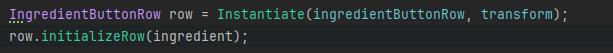
\includegraphics[width=0.8\textwidth,height=\textheight,keepaspectratio]{figures/chapter_1/prefabInstantiate.png}
    \caption{Esempio di creazione di un Prefab}
\end{figure}

Nella figura sopra vediamo un esempio di creazione di un Prefab tramite la funzione \textbf{Instantiate}, che prende come parametro il Prefab da istanziare, nel nostro caso ingredientButtonRow, e il padre in cui posizionarlo (transform). Il Prefab viene poi assegnato ad un oggetto di tipo IngredientButtonRow in modo tale da poter accedere ai suoi metodi e inizializzarlo, cosa fatta nella riga successiva. \cite{UnityPrefabs}


\subsection{IEnumerator e Coroutine}
Le Coroutine sono un modo per eseguire codice in modo asincrono, permettendo di sospendere l'esecuzione di uno script per un certo periodo di tempo senza bloccare il thread principale. Questo è particolarmente utile per operazioni che richiedono del tempo. Per eseguire una Coroutine, si utilizza il metodo \textbf{StartCoroutine}, passando come parametro un metodo che restituisce un oggetto di tipo IEnumerator.
\begin{figure}[H]
    \centering
    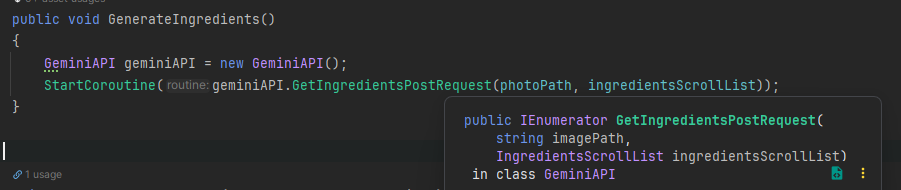
\includegraphics[width=0.8\textwidth,height=\textheight,keepaspectratio]{figures/chapter_1/UnityIEnumeratorCoroutine.png}
    \caption{Esempio di utilizzo di Coroutine}
\end{figure}

\subsection{Singleton}
Il \textbf{Singleton} è un design pattern che garantisce che una classe abbia una sola istanza fornendo un punto di accesso globale a essa. Ci sono diversi modi per implementare un Singleton in C\#, tra cui l'implementazione basica e quella thread-safe, utilizzata in questo progetto. La versione thread-safe garantisce che l'istanza sia creata in modo sicuro anche in un ambiente multi-thread, evitando problemi di concorrenza.\\Tralasciando la versione normale, la versione thread-safe utilizza un blocco chiamato nel codice \textbf{padlock} per garantire che solo un thread alla volta possa accedere alla creazione dell'istanza. 
\vspace{10cm}

Di seguito un esempio di implementazione di un Singleton thread-safe in C\#:

\begin{lstlisting}[language=java]
public sealed class Singleton
{
    private static Singleton instance = null;
    private static readonly object padlock = new object();

    Singleton()
    {
    }

    public static Singleton Instance
    {
        get
        {
            lock (padlock)
            {
                if (instance == null)
                {
                    instance = new Singleton();
                }
                return instance;
            }
        }
    }
}


\end{lstlisting}
\cite{SingletonPatternCSharp}